\documentclass{article}

\usepackage[left=2cm,right=2cm,top=2cm,bottom=2cm]{geometry} 

\usepackage[utf8]{inputenc}   % otra alternativa para los caracteres acentuados y la "ñ"
\usepackage[           spanish % para poder usar el español
                      ,es-tabla % para los captions de las tablas
                       ]{babel}   
\decimalpoint %para usar el punto decimal en vez de coma para los números con decimales

%\usepackage{beton}
%\usepackage[T1]{fontenc}

\usepackage{parskip}
\usepackage{xcolor}

\usepackage{caption}

\usepackage{fancyvrb}

\usepackage{enumerate} % paquete para poder personalizar fácilmente la apariencia de las listas enumerativas

\usepackage{graphicx} % figuras
\usepackage{subfigure} % subfiguras

\usepackage{amsfonts}
\usepackage{amsmath}

\usepackage[formats]{listings}
\lstdefineformat{R}{~=\( \sim \)}
\lstset{basicstyle=\ttfamily,format=R}

\definecolor{gris}{RGB}{220,220,220}
	
\usepackage{float} % para controlar la situación de los entornos flotantes

\restylefloat{figure}
\restylefloat{table} 
\setlength{\parindent}{0mm}


\usepackage[bookmarks=true,
            bookmarksnumbered=false, % true means bookmarks in 
                                     % left window are numbered
            bookmarksopen=false,     % true means only level 1
                                     % are displayed.
            colorlinks=true,
            allcolors=blue,
            urlcolor=blue]{hyperref}
\definecolor{webblue}{rgb}{0, 0, 0.5}  % less intense blue


\title{\Huge SWAP: Asegurar la granja web\vspace{10mm}}

\author{\huge David Cabezas Berrido \vspace{10mm} \\ 
  \huge dxabezas@correo.ugr.es \vspace{10mm}}

\begin{document}
\maketitle
\tableofcontents
\newpage

\section{Instalar un certificado SSL autofirmado para configurar el acceso por HTTPS}

Toda esta sección la haremos en la máquina 1.

Para habilitar el módulo SSL de Apache2, ejecutamos la siguiente línea.

\begin{Verbatim}[tabsize=4]
sudo a2enmod ssl 
\end{Verbatim}
Habilita el módulo y sus dependencias. Salida:
\begin{Verbatim}[tabsize=4]
Considering dependency setenvif for ssl:
Module setenvif already enabled
Considering dependency mime for ssl:
Module mime already enabled
Considering dependency socache_shmcb for ssl:
Enabling module socache_shmcb.
Enabling module ssl.
See /usr/share/doc/apache2/README.Debian.gz on how to configure SSL and create self-signed certificates.
To activate the new configuration, you need to run:
systemctl restart apache2
\end{Verbatim}
Restauramos el servicio con \verb^sudo systemctl restart apache2^. Ahora creamos una carpeta para los certificados de Apache, y creamos un par de clave y cerficiado. Le ponemos longitud de clave 2048 bits y 365 de validez.

\begin{figure}[H]
	\centering
	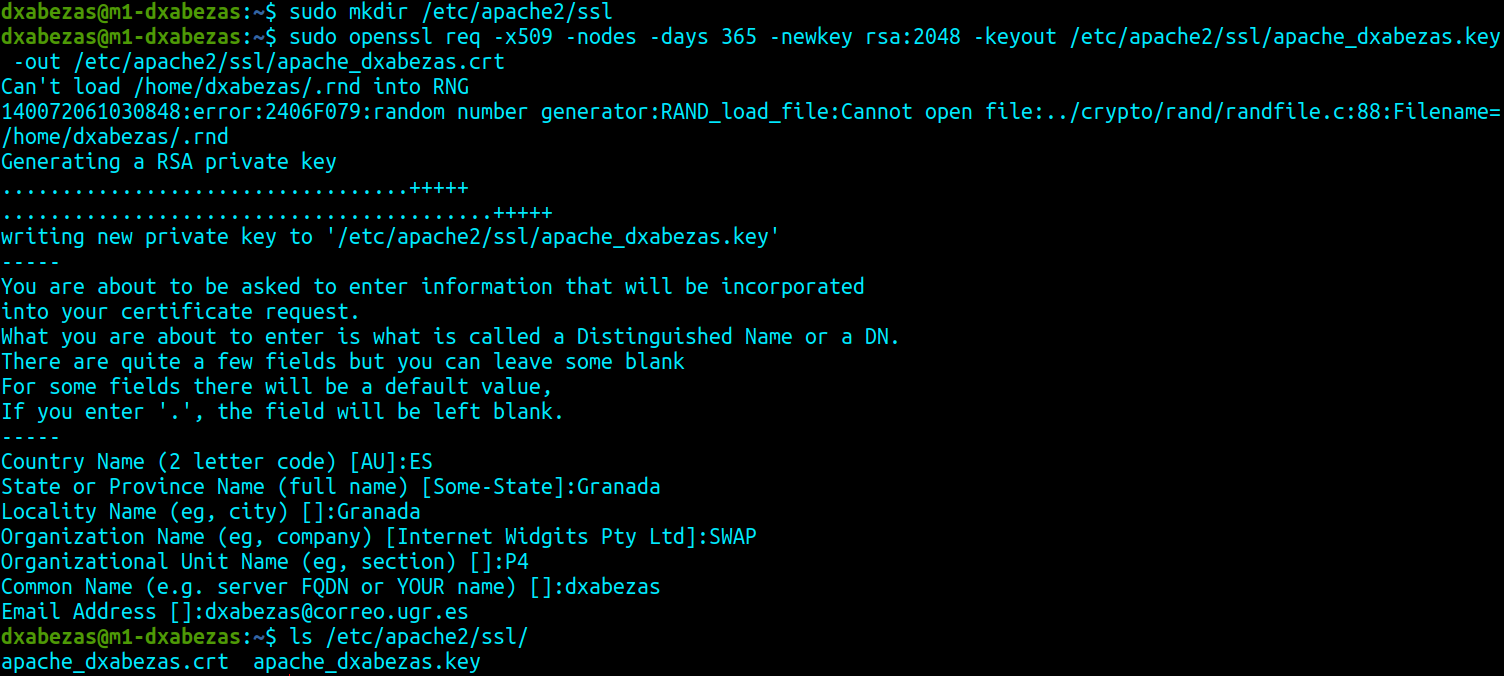
\includegraphics[width=180mm]{imgs/cert-create}
	\caption{Rellenamos los datos del certificado como se indica en el guión. Comprobamos que se ha creado el par correctamente.}
	\label{fig:cert-create}
\end{figure}

Como opciones avanzadas comentamos que \texttt{-x509} auto-firma el certificado, se obtendría una solicitud de certificado si no usásemos
esta opción. Además, la opción \\ \texttt{-subj "/C=TheCountry/CN=theCommonName/ST=theState/O=theOrganization/..."} permite especificar los datos
desde la orden, pueden consultarse las abreviaturas en \href{https://stackoverflow.com/questions/6464129/certificate-subject-x-509}
este post se encuentran los distintos atributos y sus abreviaturas.

Ahora modificamos el fichero de configuración \texttt{/etc/apache2/sites-available/default-ssl.conf}, tenemos que tener el siguiente
bloque (\verb|SSLEngine on| ya estaba puesto).

\begin{Verbatim}[tabsize=4]
#   SSL Engine Switch:
#   Enable/Disable SSL for this virtual host.
SSLEngine on
SSLCertificateFile /etc/apache2/ssl/apache_dxabezas.crt
SSLCertificateKeyFile /etc/apache2/ssl/apache_dxabezas.key
\end{Verbatim}
También tenemos que comentar las líneas que sobreescriben estas directivas más abajo. Guardamos los cambios y ejecutamos
\begin{Verbatim}[tabsize=4]
sudo a2ensite default-ssl
sudo service apache2 reload
\end{Verbatim}

Cuando accedemos a la página, nos avisa de que es insegura porque el certificado es auto-firmado. Debemos permitir la excepción en
el navegador o añadir \texttt{-k} con \texttt{curl}. Si le damos al candado junto a la dirección y a \texttt{More Information},
podemos visualizar el certificado que hemos creado.

\begin{figure}[H]
	\centering
	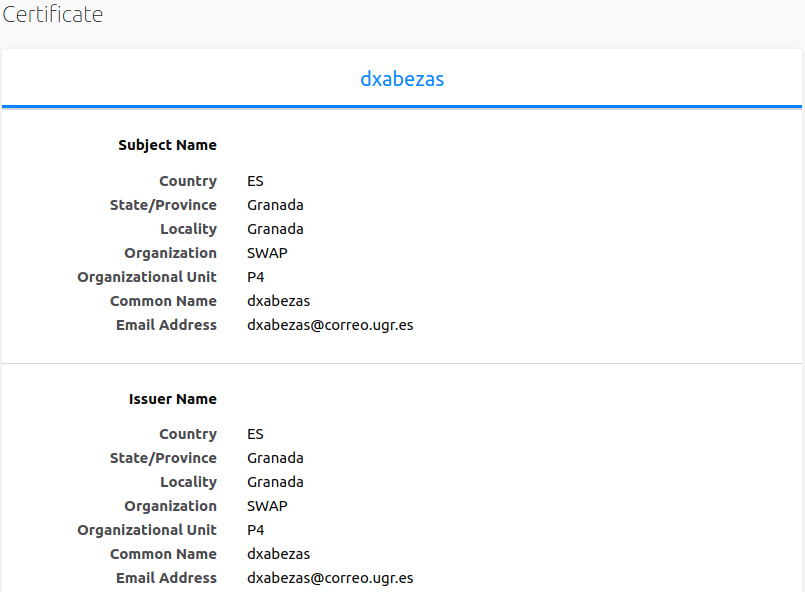
\includegraphics[width=140mm]{imgs/cert-view}
	\caption{Certificado con los datos que hemos creado.}
	\label{fig:cert-view}
\end{figure}

Como opciones avanzadas, mostramos como obtener el certificado sin ayuda del navegador, con \texttt{openssl}:
\begin{Verbatim}[tabsize=4]
openssl s_client -connect 192.168.56.101:443 -showcerts
\end{Verbatim}

También hay varias opciones adicionales en la configuración de Apache2 SSL. Se activan con
\begin{Verbatim}[tabsize=4]
SSLOptions +opcion1 +opcion2
\end{Verbatim}

Por ejemplo, cuando se trabaja con autenticación y se requiere que los clientes también tengan certificados, la opción
\texttt{FakeBasicAuth} requiere que los clientes pongan el campo Subject the su certificado como usuario, la contraseña siempre
es la misma: ``xxj31ZMTZzkVA'' (que es una encriptación por DES de la palabra ``password''), por ello el nombre de Fake.

\section{Configurar la granja web para que permita HTTPS}

Primero replicamos la configuración en la máquina 2. En lugar de crear un nuevo certificado, copiamos el de M1.
Desde M1:
\begin{Verbatim}
sudo scp /etc/apache2/ssl/apache_dxabezas.crt dxabezas@192.168.56.102:/home/dxabezas/apache_dxabezas.crt
sudo scp /etc/apache2/ssl/apache_dxabezas.key dxabezas@192.168.56.102:/home/dxabezas/apache_dxabezas.key
\end{Verbatim}

Ahora desde M2:
\begin{Verbatim}
sudo mkdir /etc/apache2/ssl
sudo mv /home/dxabezas/apache_dxabezas.* /etc/apache2/ssl/
sudo a2enmod ssl & sudo service apache2 restart
sudo nano /etc/apache2/sites-available/default-ssl.conf
\end{Verbatim}

Escribimos las líneas 
\begin{Verbatim}
SSLCertificateFile /etc/apache2/ssl/apache_dxabezas.crt
SSLCertificateKeyFile /etc/apache2/ssl/apache_dxabezas.key
\end{Verbatim}
y comentamos las equivalentes que ya había. Terminamos con 
\begin{Verbatim}[tabsize=4]
sudo a2ensite default-ssl
sudo service apache2 reload
\end{Verbatim}

Cuando nos conectamos a M2 desde el navegador por HTTPS obtenemos el mismo resultado, y también podemos visualizar el mismo
certificado.

Falta configurar M3. Otra vez desde M1 copiamos el certificado:

\begin{Verbatim}
sudo scp /etc/apache2/ssl/apache_dxabezas.crt dxabezas@192.168.56.103:/home/dxabezas/apache_dxabezas.crt
sudo scp /etc/apache2/ssl/apache_dxabezas.key dxabezas@192.168.56.103:/home/dxabezas/apache_dxabezas.key
\end{Verbatim}

Y desde M3:
\begin{Verbatim}
mv apache_dxabezas.* ssl/
sudo nano /etc/nginx/conf.d/default.conf
\end{Verbatim}

Y creamos un nuevo server como se indica en el guión:

\begin{Verbatim}[tabsize=4]
server {
	listen 443 ssl;
	ssl on;
	ssl_certificate         /home/dxabezas/ssl/apache_dxabezas.crt;
	ssl_certificate_key     /home/dxabezas/ssl/apache_dxabezas.key;
	server_name balanceador_dxabezas;
	access_log /var/log/nginx/balanceador_dxabezas.access.log;
	error_log /var/log/nginx/balanceador_dxabezas.error.log;
	root /var/www/;
	
	location /
	{
		proxy_pass http://balanceo_dxabezas;
		proxy_set_header Host $host;
		proxy_set_header X-Real-IP $remote_addr;
		proxy_set_header X-Forwarded-For $proxy_add_x_forwarded_for;
		proxy_http_version 1.1;
		proxy_set_header Connection "";
	}
}
\end{Verbatim}
Tras restaurar NGINX, podemos acceder desde el navegador por HTTPS a la IP de M3 de la misma forma que hacíamos con
M1 y M2 (se marca como insegura y hay que añadir una excepción). Una vez entramos, M1 y M2 se turnan para servirnos
su \texttt{index.html}. También podemos ver el mismo certificado tal y como hacíamos antes.

Al igual que antes, todas las máquinas aceptan también tráfico HTTP.

Como opciones avanzadas, comentaremos \href{http://nginx.org/en/docs/http/ngx_http_ssl_module.html#ssl_protocols}{protocolos} y 
\href{http://nginx.org/en/docs/http/ngx_http_ssl_module.html#ssl_ciphers}{cifrados} para SSL. 

Dentro del archivo de configuración del server (NGINX), la directiva \texttt{ssl\_protocols} limita las conexiones a las compatibles con
las versiones de SSL y TLS que indiquemos de la siguiente lista: SSLv2, SSLv3, TLSv1, TLSv1.1, TLSv1.2, TLSv1.3.
Por defecto, las versiones que se aceptan son las de este ejemplo:
\begin{Verbatim}
ssl_protocols TLSv1 TLSv1.1 TLSv1.2;
\end{Verbatim}

Igualmente, la directiva \texttt{ssl\_ciphers} limita las conexiones a las compatibles con los sistemas de cifrado que se especifiquen,
deben escribirse en un formato entendiblel por OpenSSL, por ejemplo:
\begin{Verbatim}
ssl_ciphers ALL:!aNULL:!EXPORT56:RC4+RSA:+HIGH:+MEDIUM:+LOW:+SSLv2:+EXP;
\end{Verbatim}

\section{Cortafuegos \emph{iptables}}


\end{document}
